\documentclass[12pt]{article}
\usepackage[utf8]{inputenc}
\usepackage{upquote}
\usepackage[margin=20mm]{geometry} 
\usepackage{amsmath,amsthm,amssymb}
\usepackage{graphicx}
\usepackage{listings}
\newenvironment{statement}[2][Statement]{\begin{trivlist}
\item[\hskip \labelsep {\bfseries #1}\hskip \labelsep {\bfseries #2.}]}{\end{trivlist}}
\usepackage{xcolor}
\usepackage{subfigure}


% Listings package for code rendering (No external dependencies)
\usepackage{listings}  
\usepackage{xcolor}   % Color support
\usepackage{tcolorbox} % Box for better appearance

% Define custom colors for code highlighting
\definecolor{codegreen}{rgb}{0,0.6,0}
\definecolor{codegray}{rgb}{0.5,0.5,0.5}
\definecolor{codepurple}{rgb}{0.58,0,0.82}
\definecolor{backcolour}{rgb}{0.95,0.95,0.92}


\lstset{frame=tb,
    language=Python,
    backgroundcolor=\color{backcolour},   
    commentstyle=\color{codegreen},
    keywordstyle=\color{magenta},
    numberstyle=\tiny\color{codegray},
    stringstyle=\color{codepurple},
    basicstyle=\ttfamily\footnotesize,
    breakatwhitespace=false,         
    breaklines=true,                 
    keepspaces=true,                 
    numbers=left,       
    numbersep=5pt,                  
    showspaces=false,                
    showstringspaces=false,
    showtabs=false,                  
    tabsize=2,
}




\title{Assignment 2}


%\author{Author \\
%  Wanjing Hu / fng685@alumni.ku.dk  \\
%  Shuangcheng Jia/   \\
%  Zhigao Yan / sxd343@alumni.ku.dk  \\
%} 
 

\begin{document}
\maketitle

\section{Pixel-wise contrast enhancement}
\subsection{Gray scale Image}
%wanjing
\begin{lstlisting}
def gamma_transform(image, gamma):
    # Normalize to [0,1]
    image = image.astype(np.float32) / 255.0 
    # Apply gamma correction
    corrected = np.power(image, gamma) 
    # Convert back to [0,255]
    return (corrected * 255).astype(np.uint8) 
\end{lstlisting}

A gamma=1 is equals to the original gray-scale picture, a gamma less than 1 makes dark regions brighter, and gamma larger than 1 darkens bright regions. This affects image contrast and detail visibility.

\begin{figure}[ht]
\centering
    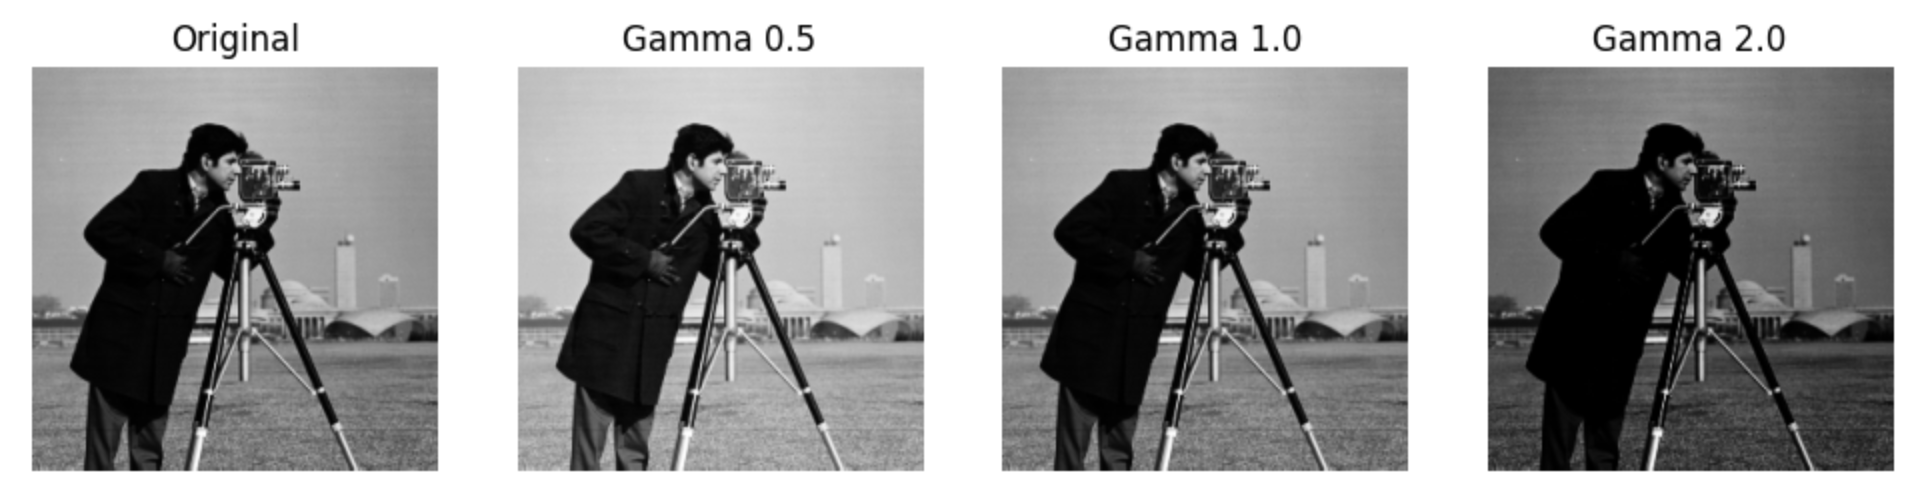
\includegraphics[width=1\columnwidth, keepaspectratio]{pics/a2-1.1}
\caption[]{Pixel-wise contrast enhancement on a gray scale picture}
\label{fig:1.1}
\end{figure}

\subsection{Color Image - RGB separately}

\subsection{Color Image - HSV color representation}

\section{Reverb Convolution}
%wanjing

\section{Image filtering and enhancement}
%zhigao

\section{Histogram-based processing}
%shuangcheng


\end{document}
